\section{Multi-authority attribute based encryption}
In this section the field of Multi-authority attribute-based encryption (MA-ABE) will be evaluated more deeply with respect to all requirements of section \ref{sec:requierements}. MA-ABE while beeing a roughly young field of ABE encryption technique enjoyed a lot of attention in the research field. 
In addition to the normal requirements like collusion resistance and revocation mechanism, MA-ABE also deals with the question on how to deescalate the global decryption power of the central authority (CA). 

A setup of a MA-ABE system looks quite similar over the field of related work. On system inizialisation we setup the CA. The purpose of the CA is to bootrap new Attribute Authoritieis (AA) which then will administer their domain. In that domain are users and attributes of this AA located. After the CA bootstraped all AAs and all users are registed it could in theority go offline. 

To ensure system wide collusion resistance each user usally gets a unique user identifiery (UID) assigned. This UID is issued by the CA which is the only entity having an overview about the whole system. 

Another notable technique recently used by \cite{yang2013dac}, \cite{wu2017security}, \cite{li2017two} and \cite{wang2011hierarchical} is \textit{proxy de-/reencryption}. It is motivated by the fact that mobile devices often don't have much computing resources so that the server may help the clients for decryption. The main idea is that the server does the preprocessing of the encrypted text given paramteres by the user. In the end the preprocessed encrypted content will be easily computable by the edge device. The cural fact is that the server will have no knowledge about the plaintext but rather helps the user on decryption or reencryption. 

In the following the different sub topics of MA-ABE will be described, analyzed given the requirement set and finally evaluated based on their perforamnce and scalability. 

\subsection{Introduction into Multi-Authority Attribute-based Encryption}
Chase 2007 \cite{chase2007multi} was the frist known to introduce the first MA-ABE schemes. In her paper she describes the process on how to derrive a multi-authority attribute-based encryption scheme vom the single authrotity schemes. 

The collussion resistance criteria in ABE implies that any data owner needs to encrypt under attributes in such kind that the ciphertext is independent of any users specific identifiers. Any user could in theory decrypter the ciphertext if he holds the fullfilling attribute set. While chase's scheme also used bilinear maps it main security was based on interpolation and the fact that no underdefined linaer equation system could definitly be solved\footnote{For LSSS matrix are based on the same assumption.}.  

Colluding users can not decrypter any cipher text and the plain text is encrypted using a blinded master secret. The blinding factor is then implemented in the policy so that any user satisfying this policy can restore the blinding factor and so revocer the plaintext. 

In the next step each user is given blinded attribute private keys so that when used on decryption the plaintext is still blinded with the user specific identifier. Using pairings this identifier can be substituted and the plaintext gets revealed. 

Two cural disadventages where not respected by chase in her initial scheme. First the CA had global decryption power. It needed to issue each AA a specific seed so that on using this seed in a pheudo random generator the CA knew what random value would be calculated. This was importent since the CA need to isse the user his private key which combined with the private attribute keys from the AA would reveal on decryption the unblinded plaintext. 

Chase improved her scheme 2009 in \cite{chase2009improving}. Now all AAs will do a n-party key exchange to distribute the secret seeds with each other. Agreeing on a well known value the CA was no longer needed and as long $N-2$ AAs are not colluding with each other the secret remained secure. 

The other disadventage, that was will present in the updated scheme, was that no new AA could be added after system inizialisation since it would trigger a new system inizialisation and distribution of the master secret. 

The lack of addition new attribute authorities and the missing revocation scheme made chases scheme impractical for further evaluations but give a good introduction the fitfalls of MA-ABE schemes.

\subsection{Decentralized attribute-based encryption}

\subsection{Efficient Data Access Control for Multi-Authority Cloud Storage}
The most explored field in MA-ABE is the Efficient Data Access Control for Multi-Authrotity Cloud Stroage (DAC-MACS) family \cite{yang2013dac}. First instroducted by Yang \textit{et. al.} 2013 it desribes an efficient, revocable MA-ABE scheme based on CP-ABE and using proxy encryption on decryption and reencryption. Furhter this scheme features a large attribute universe, adding AAs on the running system and serves with a CA that has no global decryption power. In sort DAC-MACS satisfy all the non-optional requirements.

DAC-MACS elliminates the need for the global decryption power of the CA by issuing $k$ ciphertexts: One per AA. \footnote{If the ciphertext does not require any attributes of an specific authority it does not have to create a ciphertext for this domain.} It does not require any coordination between authorities which enables to add new AAs at runtime without recreating the user keys. This scheme also includes features for efficient revocation while it claims to maintain forward and backward secrecy.

DAC-MACS is not collusion resistance on attribute revocation under the active attack model. The scheme NEDAC-MACS (New Extended DAC-MACS) shows and solves this vulnerability \cite{wu2017security}. Recent studies introduce a more efficient, scalable and secure approaches such as MAACS \cite{li2016secure} and TFDAC-MACS (Two-Factor DAC-MACS)\cite{li2017two}. 

All the DAC-MACS schemes are structed in the same way. They usally describe six different entities:

\begin{enumerate}
	\item \textbf{Certificate/Central Authority (CA)} The purpose of the CA is to issue user their global identifier (GID). Furhter they bootstrap the different AAs. The CA remains trusted but do not have any decryption power in the system. 
	\item \textbf{Attribute Authority (AA)} A attribute authority administers their domain. Issues attributes and their respective privat key to the user. They only accept a user if his GID is signed by the CA. 
	On revocation they will need to update the users secret keys as well as the ciphertext encrypted with the revoked attribute key. AAs are assumed to be trusted but can be compromised by an adversary.
	\item \textbf{Server} The purpose of the server is to help the user with proxy re- and decryption. If an AA broadcast a revocation of an attribute, the server may download all related ciphertexts from the CSP to update them with the new attribute. 
	Further, the user may give the server his attribute privat keys so that the server can pre compute the ciphertext. Usally the thread model for the server is honest-but-curious. Please note, that the CA and the server are two seperated entities that do not cooperate.
	\item \textbf{Data owner} The data owner are usally users who want to encrypt content with under a specific access policy. To do so they use the publically available public keys pinned on the public bullition board of the respective AA. Data owner do not have any knowledge about GID or user groups in the system. After encryption they update the encrypted content to the CSP.
	\item \textbf{Cloud storage provider (CSP)} The cloud storage provider are assumed to be untrusted while they still follow the protocol. That why they only receive encrypted data. They only purpose is to store the ciphertext and make them puplically available. No authentication checks are needed.
	\item \textbf{Users} Users exist in two groups: Revoked and non-revoked. Revoked user try to collude with each other to get a higher level of decryption power. They download the files of the CSP and try to decrypter them. Only if they attribute set matches the policy of the ciphertext they will be able to decrypt the file. 
	Revoked user on the other hand try to still decipher ciphertext. In some cases they try to collude with non-revoked user to intercept the key update key to restore their decryption rights. 
	User are in general untrusted.
\end{enumerate} 

\subsection{Comparison}
\begin{figure*}[!ht]
\centering
    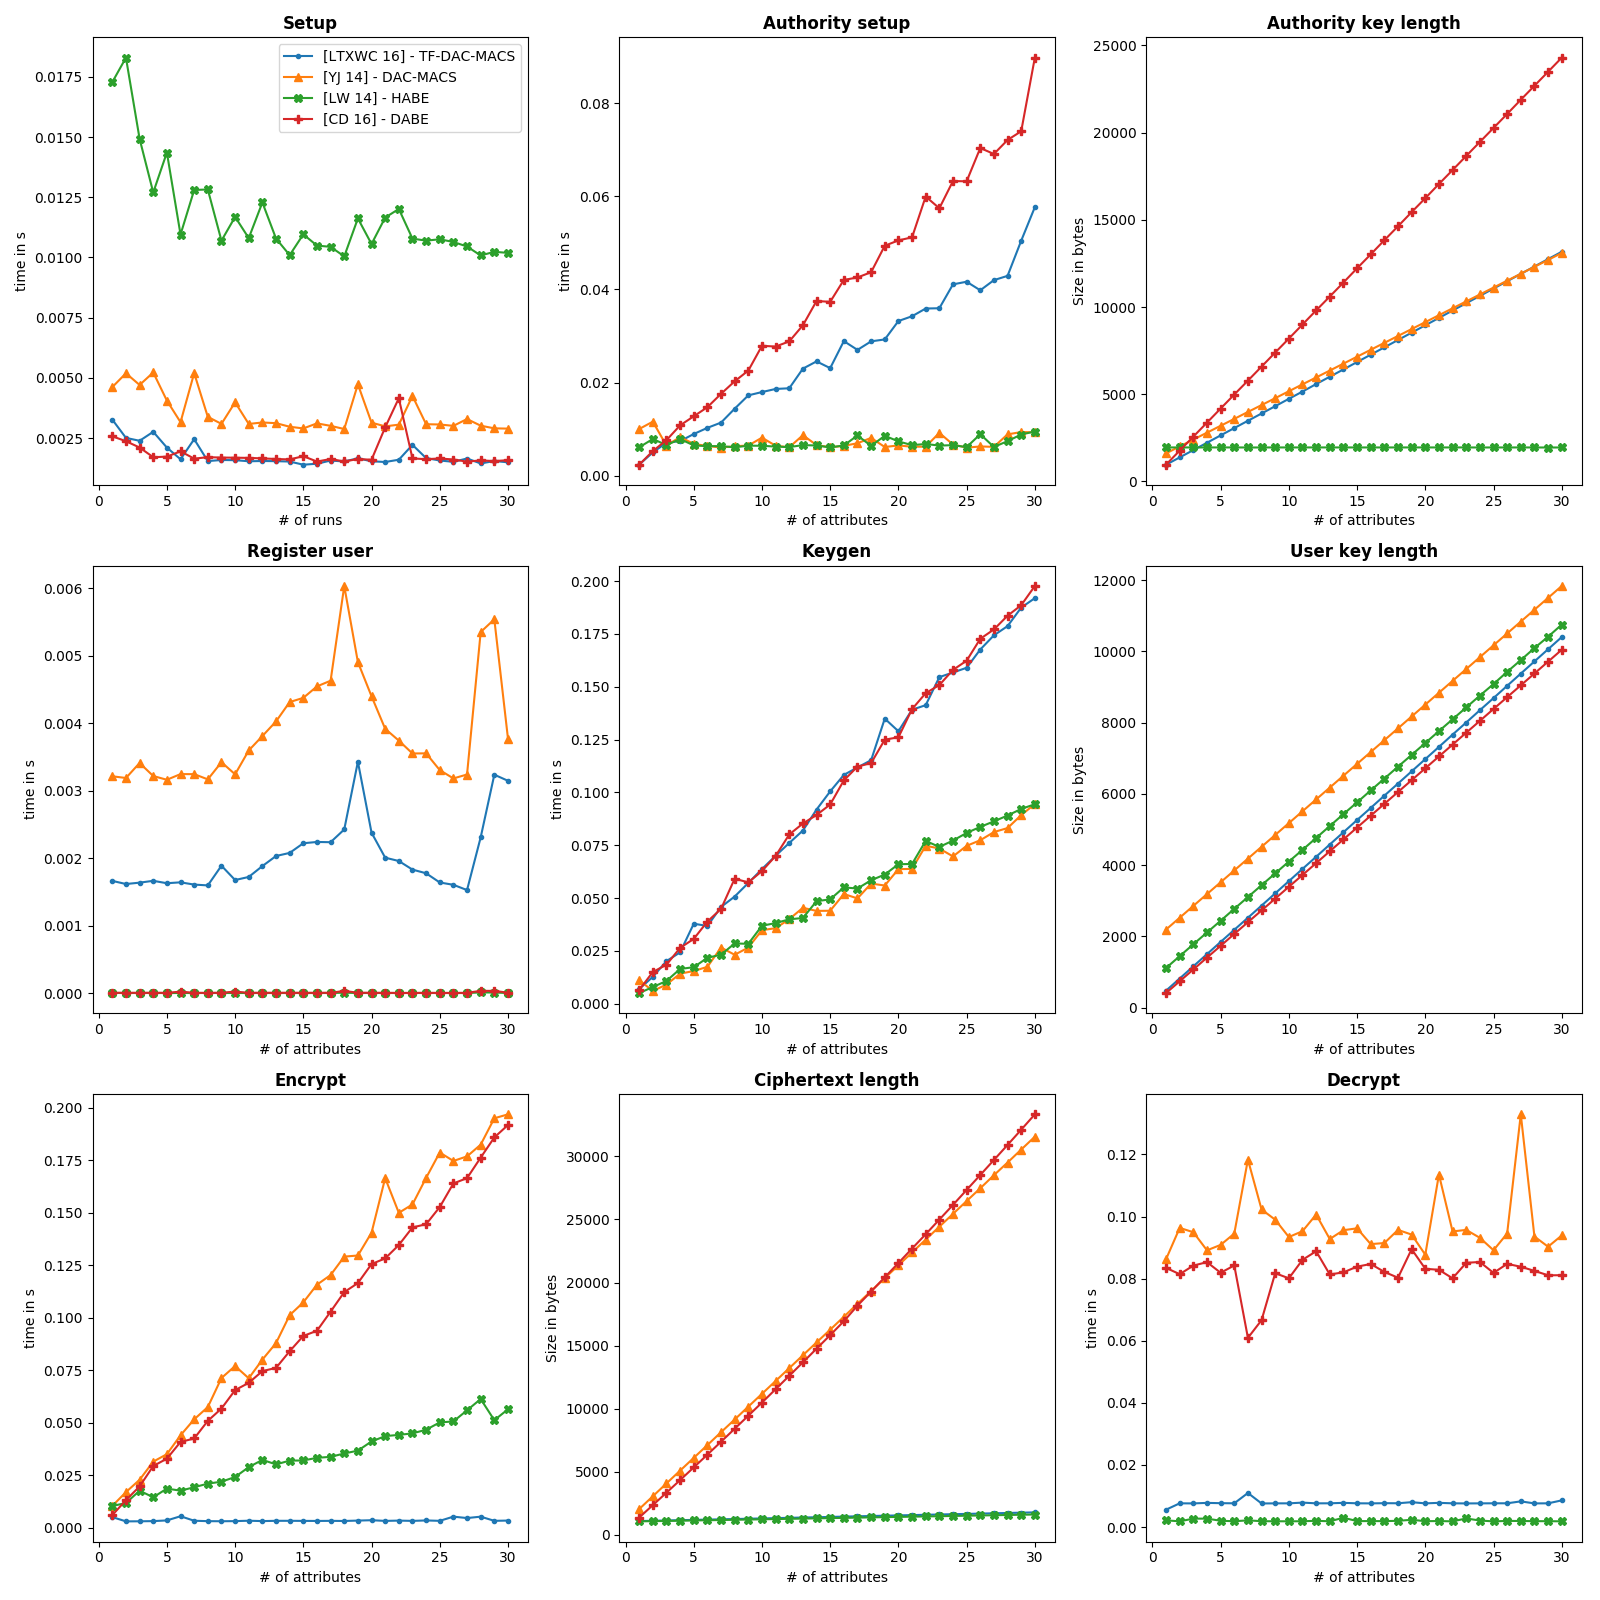
\includegraphics[width=1\linewidth]{img/maabe_comparisons.png}
    \caption{...}
    \label{fig:maabe_comparison}
\end{figure*}